\documentclass[aspectratio=169]{beamer}

\usepackage[english]{babel}
\usepackage{microtype}
\usepackage{graphicx}
\usepackage[utf8]{inputenc}
\usepackage{amssymb,amsmath}
\usepackage{resizegather}
\usepackage{ulem}
\usepackage{epsfig}
\usepackage{color}
\usepackage{contour }
\usepackage{colortbl}
\usepackage{mystyl}
% \usepackage[style=phys,articletitle=false,maxnames=4,minnames=3]{biblatex}
% \bibliography{databank}
\usepackage[font=small]{caption}
\usepackage{chemfig}
\usepackage{multimedia}
% \usepackage{animation}
\usepackage{units}
\usepackage{upgreek}
\usepackage{algorithmicx}
\usepackage{algpseudocode}
\usepackage{epigraph}
\usepackage{tipa}
\usepackage{amsthm}
\usepackage{amscd}
\usepackage{wasysym}
\usepackage{subcaption}
\usepackage{soul}
\usepackage{tikz}
\def\checkmark{\tikz\fill[scale=0.4](0,.35) -- (.25,0) -- (1,.7) -- (.25,.15) -- cycle;}

\usepackage{setspace}
\newcommand{\leftcumulant}{{\langle\langle}}
\newcommand{\rightcumulant}{{\rangle\rangle}}

% Variable width example block
\newenvironment<>{varexampleblock}[2][0.9\textwidth]{%
  \setlength{\textwidth}{#1}%
  \setlength{\linewidth}{\textwidth}%
  \begin{actionenv}#3%
    \def\insertblocktitle{#2}%
    \par%
    \setbeamercolor{local structure}{parent=example text}%
    \usebeamertemplate{block example begin}}
  {\par%
    \usebeamertemplate{block example end}%
  \end{actionenv}
}

\graphicspath{{../figures/}}
\usetheme{Luebeck}
\usecolortheme{own}

\captionsetup[subfigure]{labelformat=empty}

\titlegraphic{
  \vspace{-2\baselineskip}
  \begin{columns}
    \begin{column}{0.16\textwidth}
      \begin{figure}
        \centering
        
\includegraphics[width=\textwidth]{schmidt}
      \end{figure}

    \end{column}
    \begin{column}{0.65\textwidth}
      \centering
      \vspace{0.5\baselineskip}
      \centering
      \begin{figure}
        \centering
        
\includegraphics[width=0.3\textwidth]{logo}
      \end{figure}
    \end{column}
    \begin{column}{0.16\textwidth}
      \begin{figure}
        \centering
        
\includegraphics[width=0.75\textwidth]{dsi}
      \end{figure}
    \end{column}
  \end{columns}
  \vfill
}

\title{AI+Science Hackathon 2025}
% \author[{\includegraphics[height=0.95em]{favicon} Ludwig Schneider (he/him)}]{Ludwig Schneider}
\institute{Eric and Wendy Schmidt AI-Postdoctoral Fellowship\\Data Science Institute University of Chicago\\supported by Schmidt Sciences, LLC}
\date{April 15th -- April 29th 2025}

\begin{document}

\frame{\titlepage\thispagestyle{empty}}
\addtocounter{framenumber}{-1}


\section*{Introduction}
\begin{frame}
  \frametitle{Welcome to the AI+Science Hackathon!}
  \begin{columns}
    \begin{column}{0.45\textwidth}
      \begin{itemize}
      \item exciting new ideas
      \item transfer models to new areas
      \item compete for a trophy
      \item 2 projects
      \end{itemize}
      \begin{exampleblock}{Characterizing New Materials using AI}
        \begin{itemize}
        \item 5 teams
        \end{itemize}
      \end{exampleblock}
      \begin{exampleblock}{Reinforcement Learning to Control Networks of Living Neurons}
        \begin{itemize}
        \item 4 teams
        \end{itemize}
      \end{exampleblock}
    \end{column}
    \begin{column}{0.4\textwidth}
      \begin{figure}
        
\includegraphics[width=0.7\textwidth]{overview}
      \end{figure}
      \begin{exampleblock}{Organizing Team}
        Adam, Aditya, Alex, Anthony, Elena, Jordan, Ludwig, Marisa, Mark, Ritesh, Rui, Stephan, Victoria, William
      \end{exampleblock}
    \end{column}
  \end{columns}
\end{frame}


\subsection{Resources}

\begin{frame}
  \frametitle{Computational Environment}
  \begin{columns}
    \begin{column}{0.5\textwidth}
      \begin{itemize}
      \item 2 project specific introductions
      \item resources on RCC Midway3
      \item 8 dedicated Nvidia A100 GPUs
        \begin{itemize}
        \item \texttt{ai4s-hackathon}
        \end{itemize}
      \item group storage
      \end{itemize}
      \texttt{/project/ai4s-hackathon/XXX}
      \begin{figure}
        
\includegraphics[width=0.4\textwidth]{qr-github}
      \end{figure}
    \end{column}
    \begin{column}{0.4\textwidth}
      {\small\url{github.com/uchicago-dsi/ai-sci-hackathon-2025}}
      \begin{figure}
        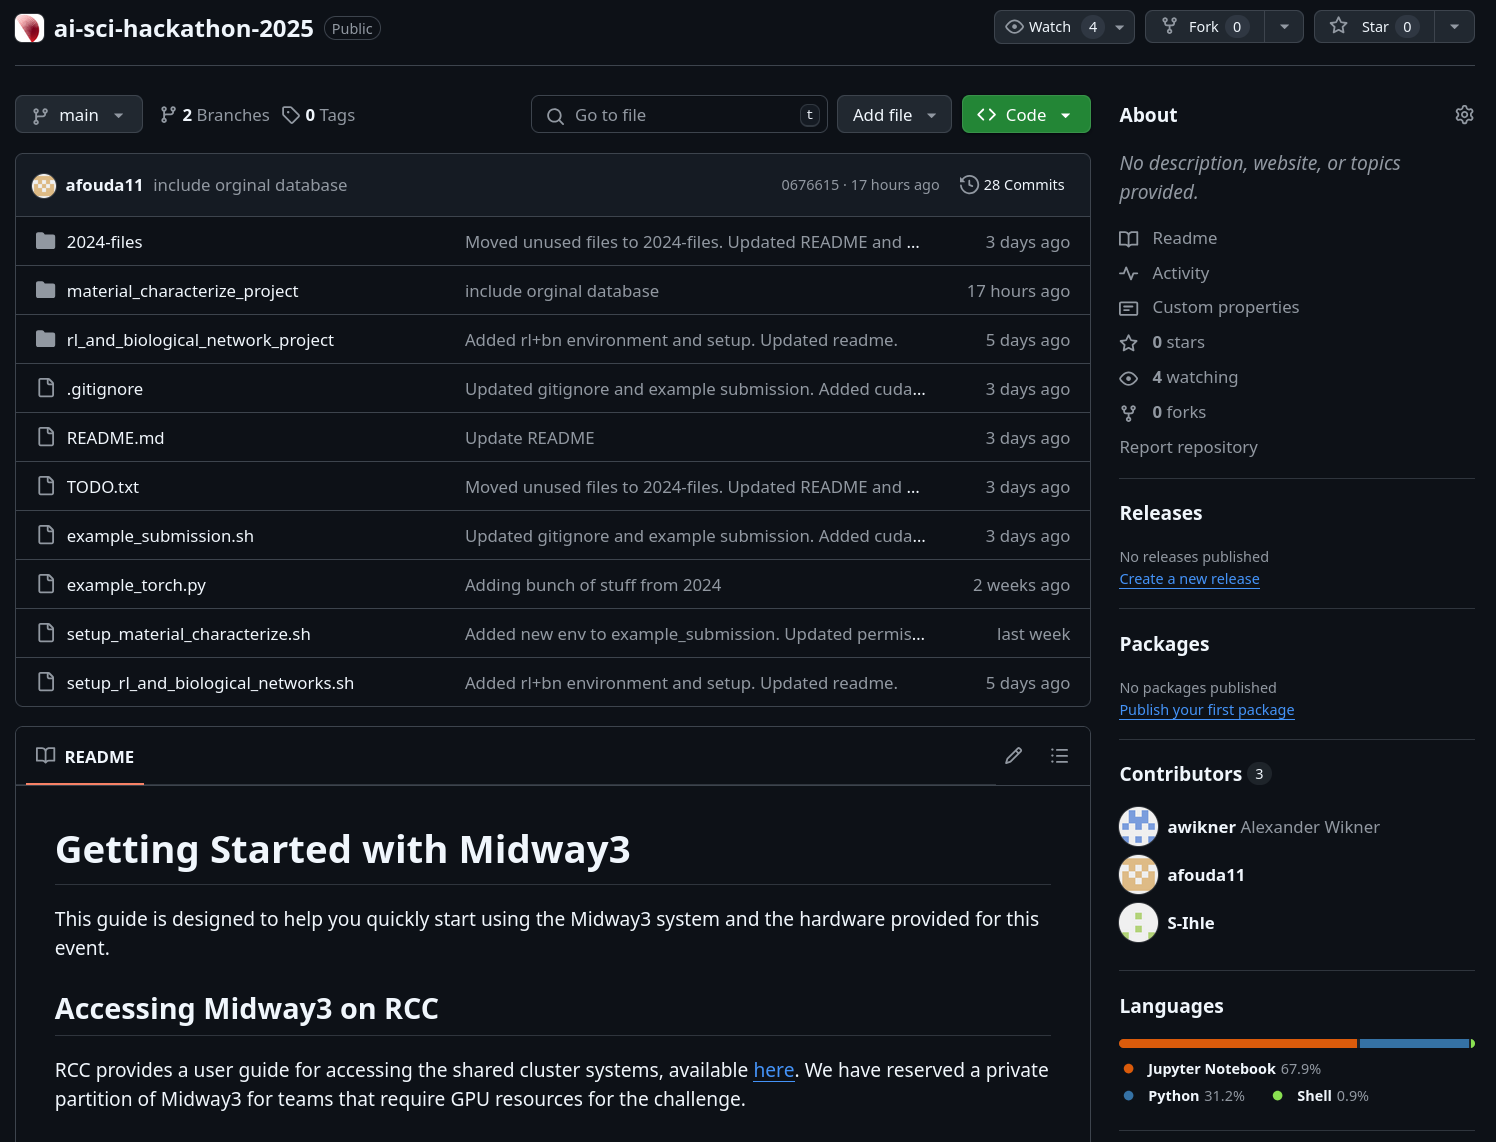
\includegraphics[width=\textwidth]{github_shot}
      \end{figure}
    \end{column}
  \end{columns}
\end{frame}

\subsection{Teams \& Mentors}

\begin{frame}
  \frametitle{Teams Selection \& Mentors}
  \begin{columns}
    \begin{column}{0.45\textwidth}
      \begin{exampleblock}{Characterizing New Materials}
      \end{exampleblock}
    \end{column}
    \begin{column}{0.45\textwidth}
      \begin{exampleblock}{Reinforcement Learning for Biological Networks}
      \end{exampleblock}
    \end{column}
  \end{columns}
  \begin{columns}
    \begin{column}{0.45\textwidth}
      \textbf{Adam}, Jordan, Rui, Elena, Ludwig, Aditya
    \end{column}
    \begin{column}{0.45\textwidth}
      \textbf{Stephan}, Madeleine, Alex, Yihang, Kyle
    \end{column}
  \end{columns}
  \begin{columns}
    \begin{column}{0.45\textwidth}
      \begin{exampleblock}{Slack Space for Communication}
        \begin{itemize}
        \item Join Slack Space
        \item Make a Group Channel
        \end{itemize}
      \end{exampleblock}
        {\tiny\url{https://join.slack.com/t/aiscienceuchi-pwb7058/shared_invite/zt-33dkfvdgm-QrNNZlG7Y0lt~2d_8uxnIw}}
        \begin{figure}
          \centering
          
\includegraphics[width=0.2\textwidth]{qr-slack}
        \end{figure}
    \end{column}
    \begin{column}{0.45\textwidth}
      \begin{exampleblock}{Getting to know your Team and Mentor}
        \begin{itemize}
        \item Check out Your Team
        \item Check out the Mentors
        \end{itemize}
      \end{exampleblock}
    \end{column}
  \end{columns}
\end{frame}

\section{Hackathon Progression}
\begin{frame}
  \frametitle{Excitement: Tuesday 15th to Thursday 17th}
  \begin{columns}
    \begin{column}{0.5\textwidth}
      \begin{itemize}
      \item get to know each other
      \item get to know your mentor
      \item brain storm model ideas
      \item pick a tech stack
      \item build a data pipeline
      \end{itemize}
      \begin{exampleblock}{Gain RCC access}
        Make sure, you successfully run a job on RCC before Thur. 17th. (Mentor)
      \end{exampleblock}
    \end{column}
    \begin{column}{0.5\textwidth}
      \begin{figure}
        
\includegraphics[width=0.9\textwidth]{day1}
      \end{figure}
    \end{column}
  \end{columns}
\end{frame}

\begin{frame}
  \frametitle{Valley of Despair: Friday 18th to Tuesday 22nd}
  \begin{columns}
    \begin{column}{0.5\textwidth}
      \begin{itemize}
      \item your first ideas didn't work
      \item the excitement is wearing off
      \item brain storm and select most promising idea
      \item iterate and build new models
      \item train new models over night
      \end{itemize}
    \end{column}
    \begin{column}{0.5\textwidth}
      \begin{figure}
        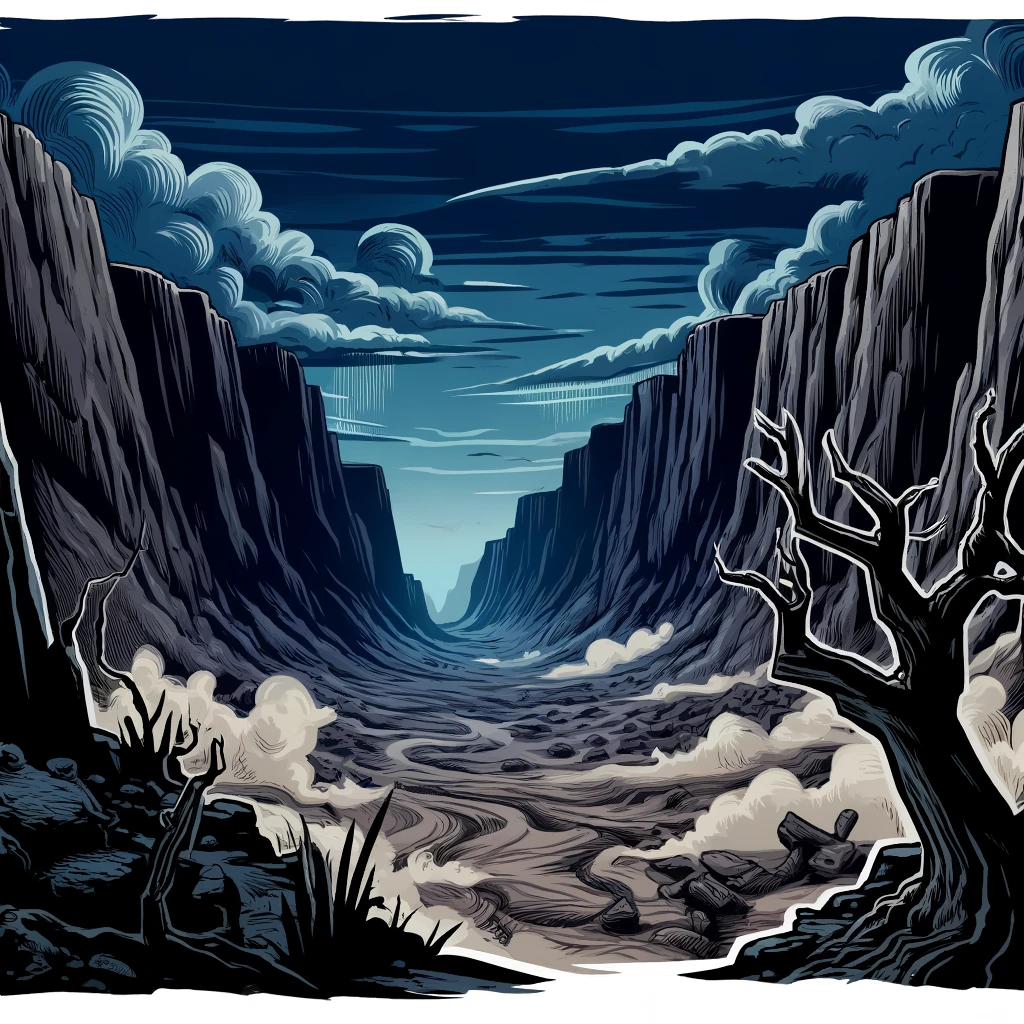
\includegraphics[width=0.9\textwidth]{day2}
      \end{figure}
    \end{column}
  \end{columns}
\end{frame}
\begin{frame}
  \frametitle{Seeing the Light: Wednesday 23rd to Monday 28th}

  \begin{columns}
    \begin{column}{0.5\textwidth}
      \begin{itemize}
      \item your models start delivering results!
      \item you can actually see how you solve this!
      \item iterate on your models
      \item optimize your hyper parameters
      \item finalize your models
      \end{itemize}
      \begin{exampleblock}{Final Results: Monday 28th}
        \begin{itemize}
        \item receive final evaluation data @ 3PM
        \item Or submit your final solution @ 3PM
        \end{itemize}
      \end{exampleblock}
    \end{column}
    \begin{column}{0.5\textwidth}
      \begin{figure}
        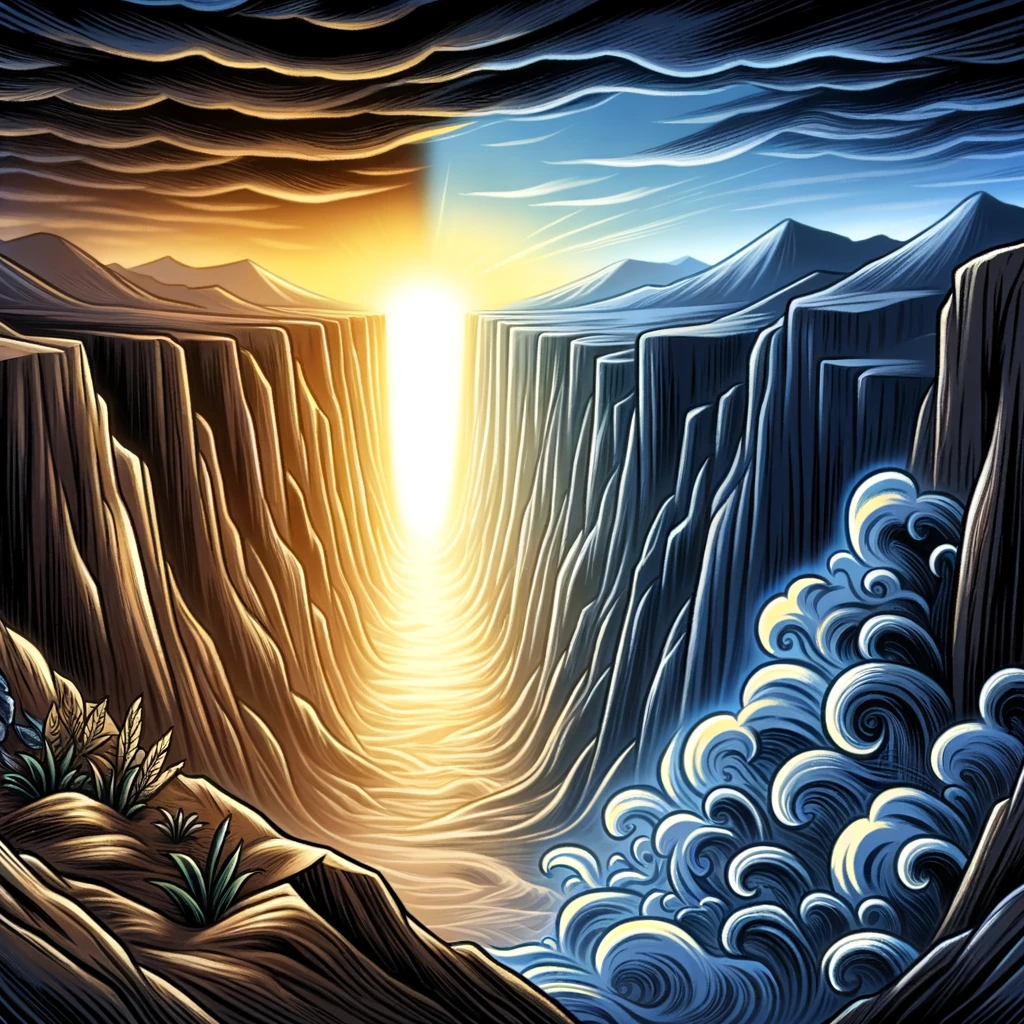
\includegraphics[width=0.9\textwidth]{day3}
      \end{figure}
    \end{column}
  \end{columns}
\end{frame}

\begin{frame}
  \frametitle{Day 4: Bringing it over the Finish Line}
  \begin{columns}
    \begin{column}{0.5\textwidth}
      \begin{itemize}
      \item gather results for last night
      \item present us your success and hiccups
      \item you have 10 minutes per team
      \item 2 minutes for questions
      \end{itemize}
      \begin{exampleblock}{Deadline}
        Presentation must be submitted 9AM \@ April 29th
      \end{exampleblock}
    \end{column}
    \begin{column}{0.5\textwidth}
      \begin{figure}
        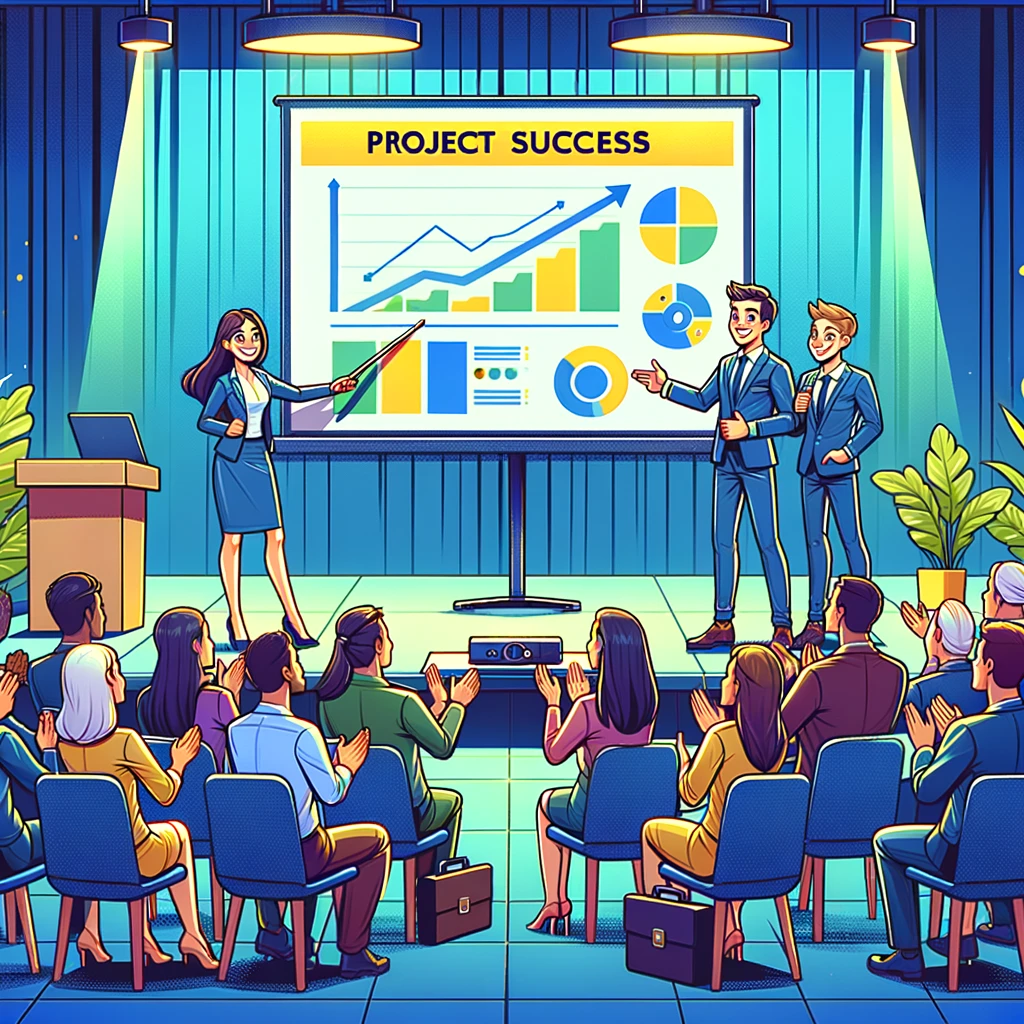
\includegraphics[width=0.9\textwidth]{day4}
      \end{figure}
    \end{column}
  \end{columns}
\end{frame}

\section{In-Person Collaboration}

\begin{frame}
  \frametitle{Teams \& Collaboration}
  \begin{columns}
    \begin{column}{0.48\textwidth}
      \begin{itemize}
      \item utilize slack!
      \item include your mentor in discussions
      \item In-Person collaboration opportunities
        \begin{table}
          \begin{tabular}{r|r|c}
            Day & Time & Room \\
            \hline
            \hline
            Tue, April 15 & 1PM -- 3PM & Searle 240A\\
            Tue, April 15 & 1PM -- 3PM & Searle 236\\
            \hline
            Thur, April 17 & 2PM -- 4PM & JCL 151 \\
            Thur, April 17 & 2PM -- 4PM & JCL 236 \\
            \hline
            Tue, April 22 & 1PM -- 3PM & Searle 240A\\
            Tue, April 22 & 1PM -- 3PM & Searle 236\\
            \hline
            Thur, April 24 & 2PM -- 4PM & JCL 151\\
            Thur, April 24 & 2PM -- 4PM & JCL 236\\
          \end{tabular}
        \end{table}
      \end{itemize}
    \end{column}
    \begin{column}{0.48\textwidth}
      \begin{figure}
        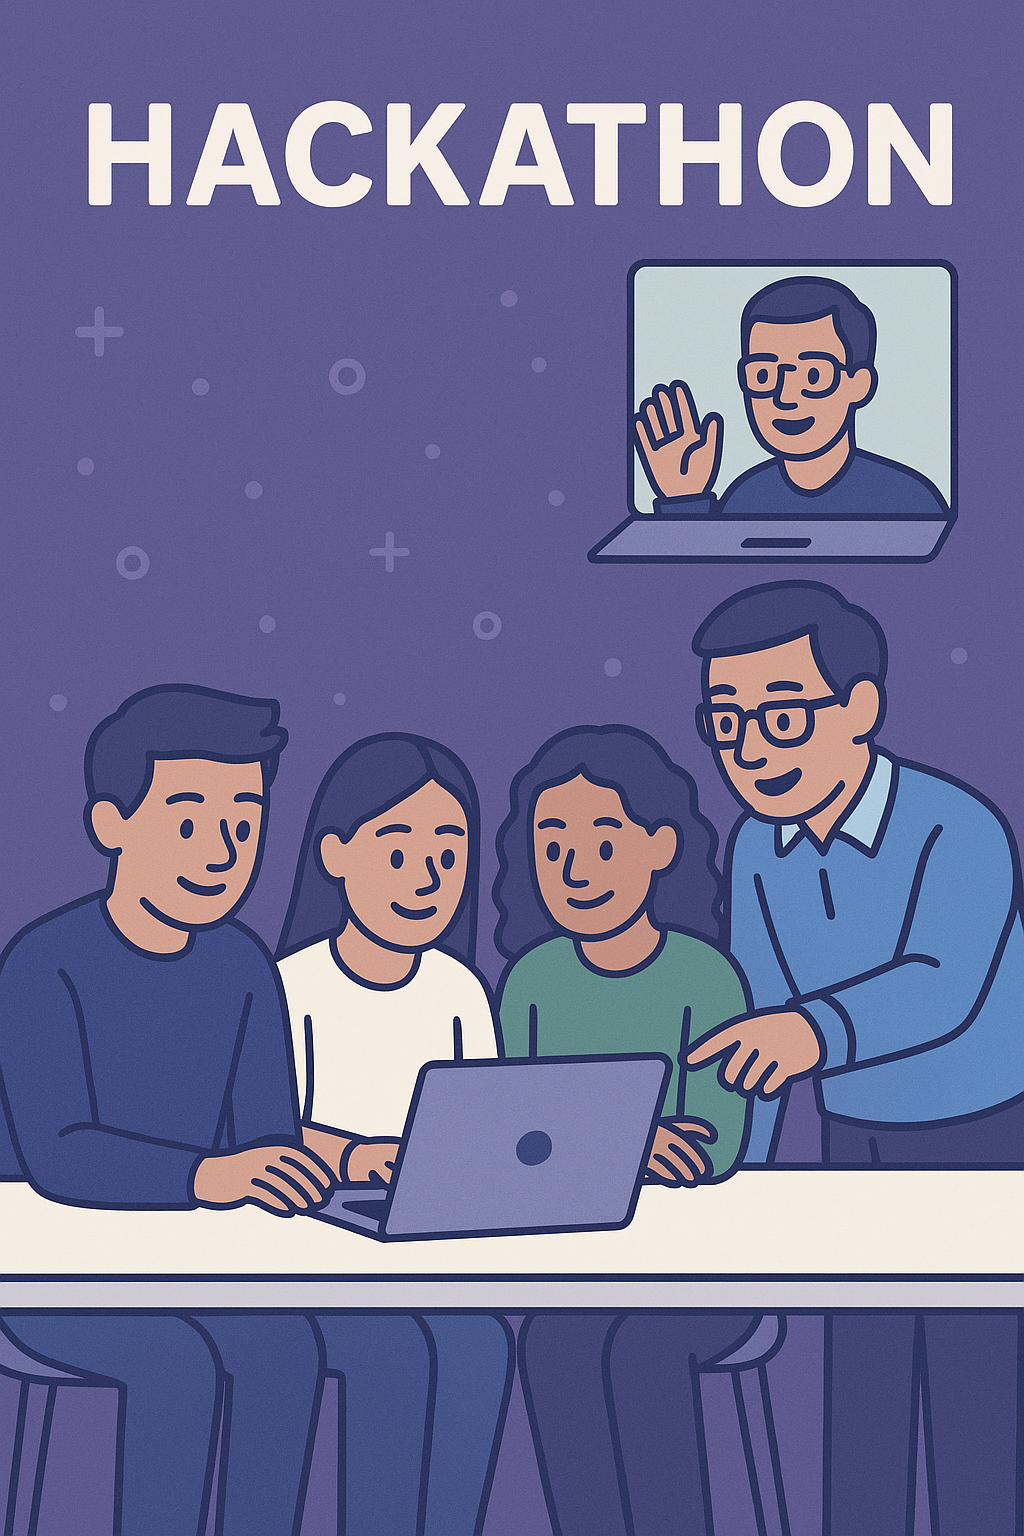
\includegraphics[width=0.5\textwidth]{collab}
      \end{figure}
    \end{column}
  \end{columns}
\end{frame}

\section{Rules}

\begin{frame}
  \frametitle{Rules for the Hackathon}
  \begin{columns}
    \begin{column}{0.45\textwidth}
      \begin{exampleblock}{\centering Play Fair!}
      \end{exampleblock}
      \begin{itemize}
      \item do not use other groups results
      \item use only the computation time you need
      \item do not use more presentation time as everyone else
      \item discuss publication with mentor and project mentor
      \end{itemize}
    \end{column}
    \begin{column}{0.5\textwidth}
      \begin{figure}
        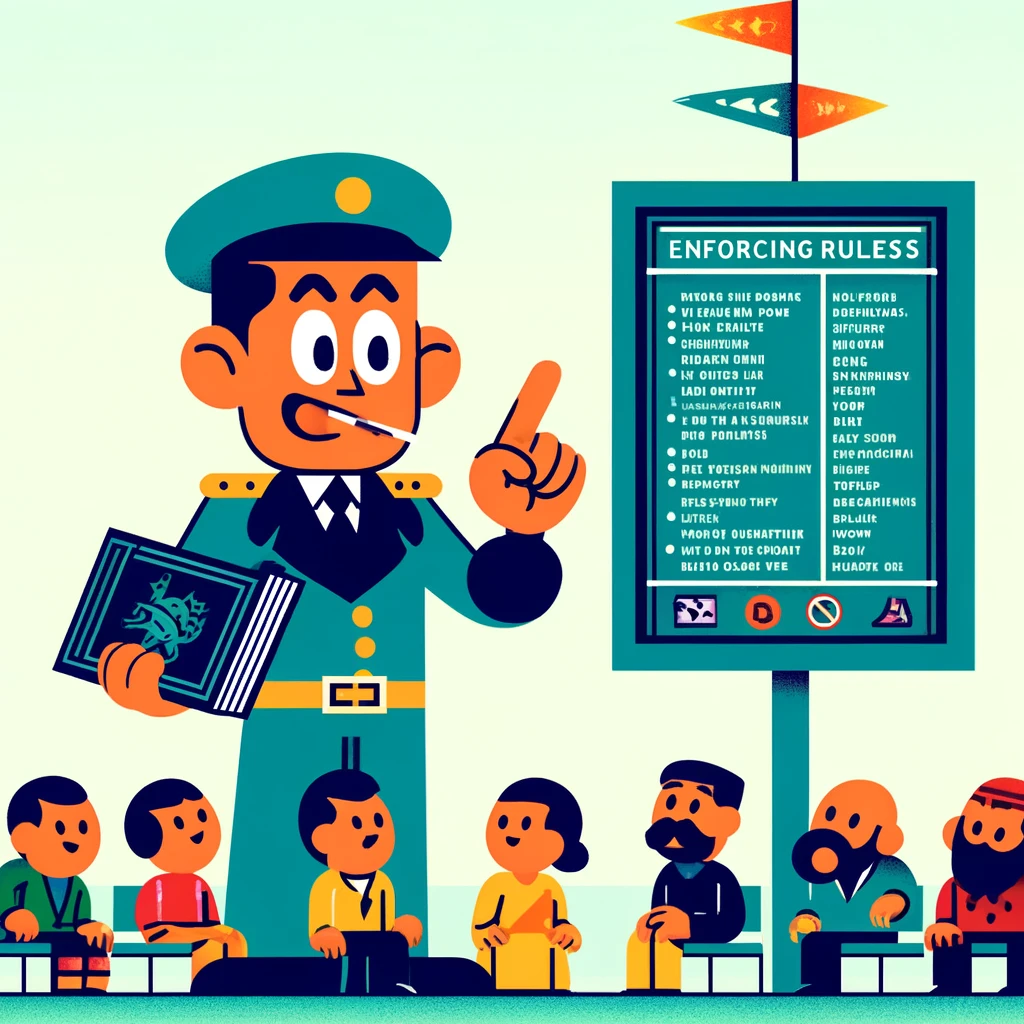
\includegraphics[width=0.9\textwidth]{rules}
      \end{figure}
    \end{column}
  \end{columns}
\end{frame}

\section*{Thank you for your attention!}
\renewcommand\Switch{0}
\renewcommand\citationtext{}
\subsection*{Questions?}

\begin{frame}
  \frametitle{Happy Hacking!}
  \centering
  {\Large Today}
  \begin{columns}
    \begin{column}{0.45\textwidth}
      \begin{exampleblock}{Characterizing New Materials using AI}
        \begin{itemize}
        \item Room: JCL 298
        \end{itemize}
      \end{exampleblock}
    \end{column}
    \begin{column}{0.45\textwidth}
      \begin{exampleblock}{Reinforcement Learning for Bio Networks}
        \begin{itemize}
        \item Room: JCL 390
        \end{itemize}
      \end{exampleblock}
    \end{column}
  \end{columns}
  \vfill
  \centering
  {\Large Thursday April 29th: 10AM}
  % \begin{columns}
  %   \begin{column}{0.45\textwidth}
  %     \begin{exampleblock}{Characterizing New Materials using AI}
  %       \begin{itemize}
  %       \item Room: JCL 298
  %       \end{itemize}
  %     \end{exampleblock}
  %   \end{column}
  %   \begin{column}{0.45\textwidth}
  %     \begin{exampleblock}{Reinforcement Learning for Bio Networks}
  %       \begin{itemize}
  %       \item Room: JCL 298
  %       \end{itemize}
  %     \end{exampleblock}
  %   \end{column}
  % \end{columns}
\end{frame}
\beginbackup


\label{fr:appendix}
\appendix

% \begin{frame}[allowframebreaks,noframenumbering]
%   \frametitle{References}
%   \printbibliography
% \end{frame}

\section{Backup slides}

\section*{The End}
\renewcommand\citationtext{}
\backupend
\end{document}

%%% Local Variables:
%%% mode: latex
%%% TeX-master: t
%%% End:
